\subsection{Methodology}
\label{sec:methodology}


%%%%%%%%%%%%%%%%%%%%%%%%%%%%%%%%%%%%%%%%%%%stats for old dataset%%%%%%%%%%%%%%%%%%%%%%%%%%%%%%%%%%%%%%%%%%%
\begin{table*}
	\centering
	\caption{Dataset summary} \label{tab-dataset-summary}
	\begin{tabular}{c|c|c|c|c|c|c}%p{0.14\textwidth}
		\hline
		% after \\: \hline or \cline{col1-col2} \cline{col3-col4} ...
		Num. of images crawled & Num. of unique images    & Num. of images downloaded  & Num. of layers downloaded \\
		\hline
		634,412                 & 457,627                 & 346,243                    & 1,763,354  \\
		\hline
		Num. of images analyzed & Num. of layers analyzed & Compressed dataset size              &  Num. of files totally \\
		\hline
		319,620                     & 1,607,533                     & 51TB                        & 117,665,791  \\
		\hline
	\end{tabular}
\end{table*}

%%%%%%%%%%%%%%%%%%%%%%%%%%%%%%%%%%%%%%%%%%%stats for new dataset%%%%%%%%%%%%%%%%%%%%%%%%%%%%%%%%%%%%%%%%%%%
%\begin{table*}
%	\centering
%	\caption{Dataset summary} \label{tab-dataset-summary}
%	\begin{tabular}{c|c|c|c|c|c|c}%p{0.14\textwidth}
%		\hline
%		% after \\: \hline or \cline{col1-col2} \cline{col3-col4} ...
%		Num. of images crawled & Num. of unique images    & Num. of images downloaded  & Num. of layers downloaded \\
%		\hline
%		634,412                 & 457,627                 & 346,243                    & 1,763,354  \\
%		\hline
%		Num. of images analyzed & Num. of layers analyzed & Compressed dataset size              &  Uncompressed dataset size \\
%		\hline
%		344,056                     & 1,748,089                     & 51TB                        & xxx  \\
%		\hline
%	\end{tabular}
%\end{table*}

%In this section we describe our methodology for obtaining a representative Docker image dataset.
%%
%(1)~obtaining a representative Docker image dataset, and
%%
%(2)~analyzing basic and deduplication properties of the dataset.
%
%%
\begin{figure}
	\centering
	% Requires \usepackage{graphicx}
	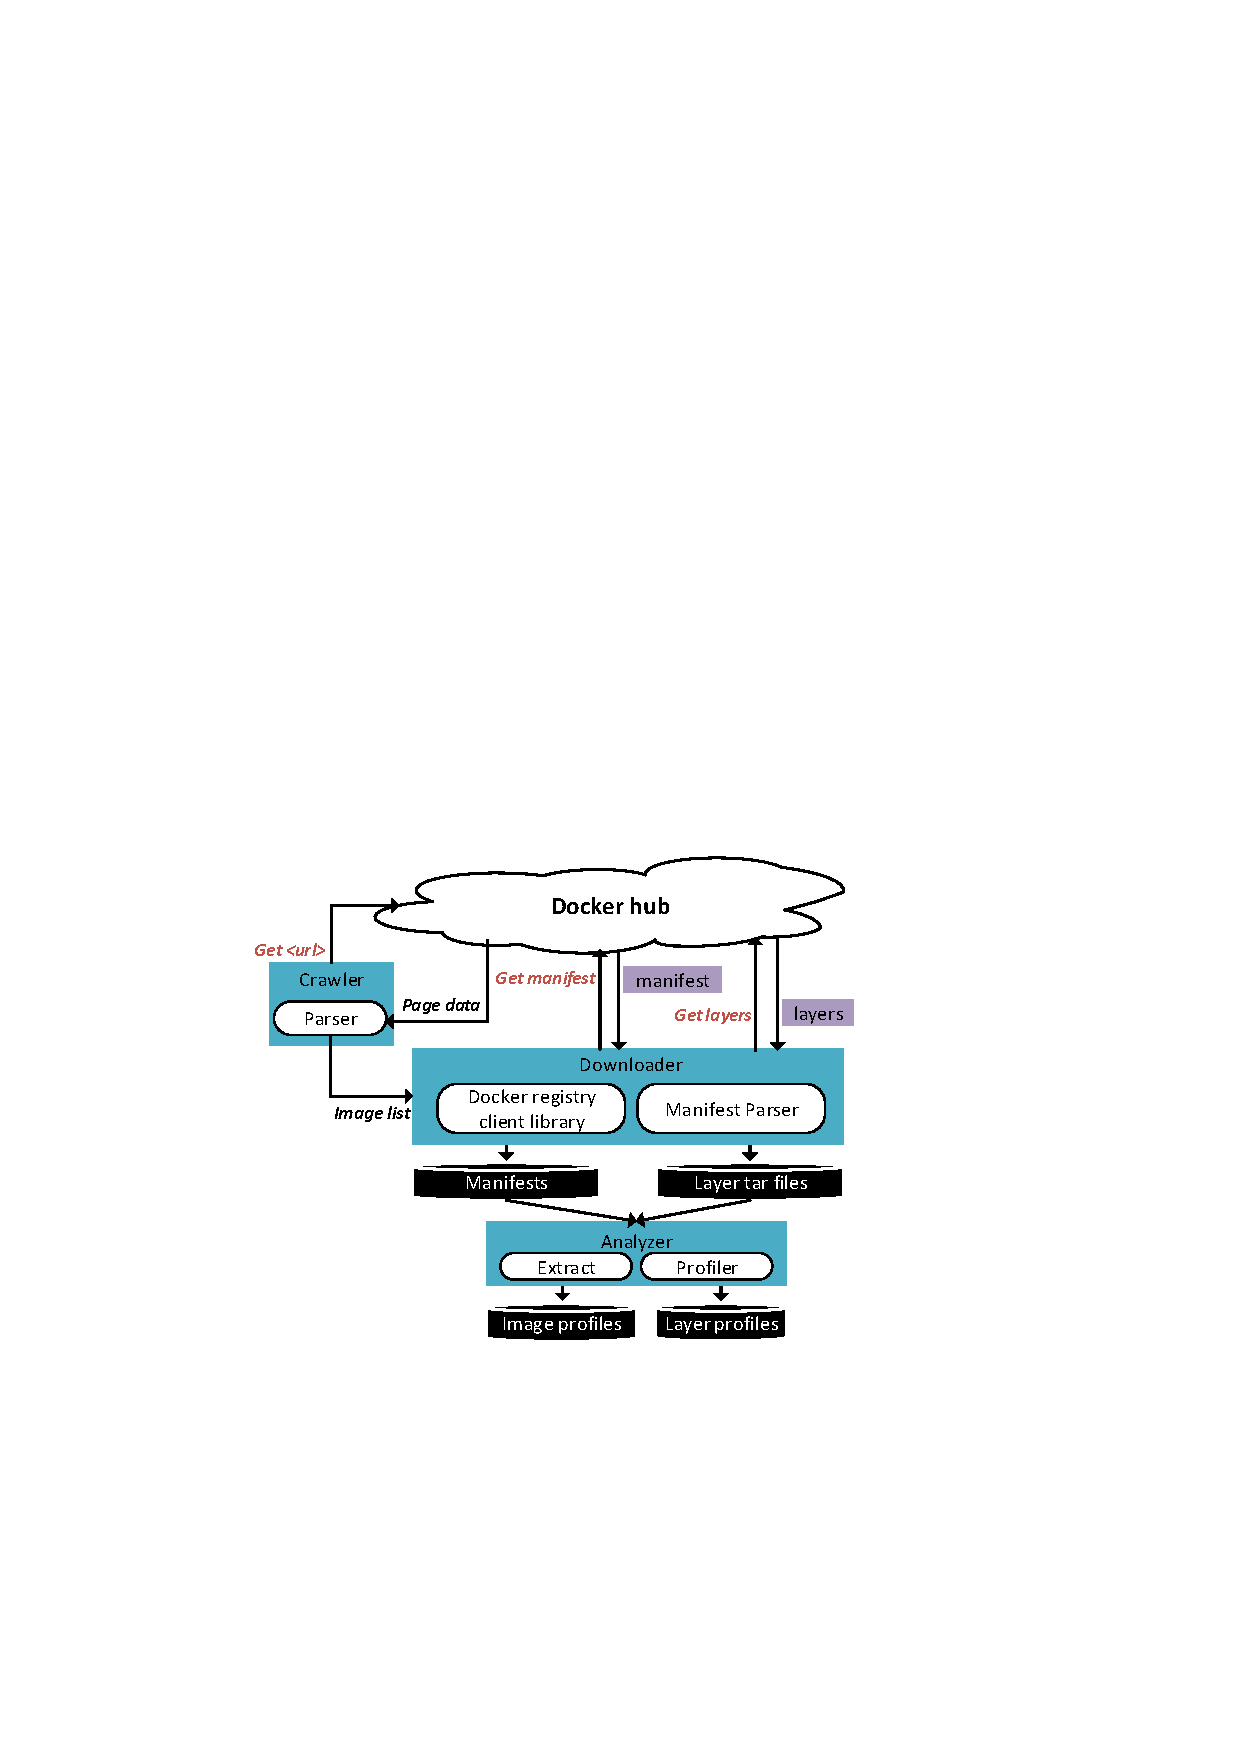
\includegraphics[width=0.5\textwidth]{graphs/fig-downloader-analyzer.pdf}\\
	\caption{Crawler, Downloader, and Analyzer
		%\vcomment{Can we add colors to this figure? Also, increase the font a bit.}
	}
	\label{fig-downloader-analyzer}
\end{figure}
%
%\subsection{Dataset acquisition}
%\label{sec:crawler}

To estimate the benefits of sub-layer deduplication for Docker registry and
identify the main sources of duplicates we downloaded a large set of
representative Docker images.
%
We chose Docker Hub~\cite{docker-hub} registry as a source of the images
because it is popular among developers and contains many public repositories.
%
We believe Docker Hub dataset is representative of other registry deployments.

To download a representative dataset from Docker Hub, 
we used web crawling to obtain a list of repositories
because Docker Hub does not provide an API to retrieve all repository names.
%
\VT{Nannan, avoid using passive voice in the sentences. E.g., above, instead of
``is needed`` you can say ``we used web crawlig to...``. Please, check the
whole text for passive voice and change where applies.}\NZ{addressed}
%
Specifically, there are two steps: i)~crawl Docker Hub web pages to list all
repositories; ii)~download the \textit{latest} image (and referenced layers)
from each repository based on the crawler results.
%
%Here, we chose latest image from each repository because (1)~the ``latest''
%version is usually the newest, stable, and commonly pulled by developers;
%(2)~downloading only the ``latest'' version can shorten our downloading
%process since the latest images already took about 30 days to download.
%
We plan to extend our analysis to other, non-``latest'', images in the future.
%
%\paragraph{Web crawler}
%
%Public repositories in Docker Hub are divided into official
%repositories---served by the Docker Hub partners---and non-official
%repositories---provided by regular users and third-party organizations.
%%
%The number official repositories is less than 200, while, the majority of
%repositories in Docker Hub are non-official (over 400 thousand).
%%
%To list non-official repositories, our crawler utilizes the Docker Hub
%web-based search engine to find all available repositories.
%%
%As the name of non-official repositories is comprised of the user name and the
%repository name separated by a ``/'', we can search for ``/'' and obtain a
%list of all non-official repositories.
%%
%The Crawler downloads all pages from the search results and parses the web
%content to build a list of all non-official repositories.
%%
%We ran the crawler on May 30th, 2017 and it produced a list of 634,412
%repositories.
%%
%After removing duplicate entries (introduced by Docker Hub indexing logic),
%the final repository list consists of 457,627 distinct repositories.
%
%\paragraph{Downloader}
%
%Instead of using the Docker client to download images, we implement our own
%downloader, which calls the Docker registry API
%directly~\cite{dockerregistryclient} to download manifests and image layers in
%parallel.
%%
%Our downloader runs significantly faster than a \texttt{docker pull}-based
%downloader because the latter one performs other operations besides
%downloading the image, such as unpacking the layers and creating the
%corresponding read-only snapshots.
%%
%Our downloader can download multiple images simultaneously and fetch the
%individual layers of an image in parallel.
%%
%Layers are transferred as gzip compressed tar archives.
%
Overall, we downloaded 47~TB of data in 355,319 image manifests with 1,792,609
compressed layers, which contains 5,278,465,130 files. 
%A total of 111,384 images could not be downloaded mainly
%because they did not have the \texttt{latest} tag.  
The downloading process took about 30 days.
%
%\vcomment{Say just one sentence why we did not download some
%images.}\nancomment{Addressed}
%
Table~\ref{tab-dataset-summary} summarizes the properties of the downloaded
dataset.
%
\VT{Let's not go into details in the table and in the text how many images we
downloaded but did not analyze, or how many we could not download, etc.  Let's
just state the total number of images/repos/layers we finally analyzed and
their sizes and file numbers.}\NZ{addressed}
%
Specifically, we built a 8-node Spark
~\cite{xxx} 
cluster with HDFS
~\cite{xxx} 
as a backend storage system
to do an in-depth analysis and save analysis results to HDFS.
\VT{Maybe mention a sentece or two that we used SPARK cluster to do the
analysis?}\NZ{addressed}

